\chapter{基于缓冲区分析的直播系统码率自适应算法}

在上一章中,我们以达尔文流媒体服务器作为平台为视频点播系统的传输过程设计了一个码率自适应算法。本章针对如今越来越流行的用户生成内容(User Generated Content, UGC)直播应用进行研究,提出了一个基于传输中缓冲区分析的码率自适应算法,来改善从数据产生设备向服务器上传数据的效率。

\section{视频直播系统概述}

在有些视频直播系统中,视频内容由服务器或者与服务器通过局域网紧密连接的设备生成。在这种情形下,视频直播和视频点播系统有很大的相似性。这时视频数据的传输主要是从服务器到观看者客户端。直播服务器将动态生成的视频数据发送给客户端,和点播最主要的区别在于传输速率不能超过视频数据生成的速率,因为当所有生成的数据都传输之后,客户端需要等待下一个数据片段就绪\supercite{Thang2014}。

但在UGC直播模式下,服务器本身不充当初始的内容产生方, 而是在其他设备上持续生成的视频内容经过互联网(具有不确定的带宽和不可忽略的延迟)传输到中转服务器,然后再由服务器分发给观看者。目前这种模式的直播越来越流行,因为已经非常普及的智能手机成为了理想的内容产生方和观看接收方。图\ref{fig:07}展示了通用的手机视频直播系统的主要模块。集成了高效视频编码器的智能手机作为内容提供者,将实时视频数据传输到服务器。服务器所在的本地网络内设有转码器和提供播放服务的内容服务器。转码服务器会将上传的码流实时转码成多路具有不同码率的视频流,交由内容服务器供不同的观看者播放。播放客户端可以根据自己的网络环境选择最合适的码率,从服务器获取视频数据。

\begin{figure}[t]
	\vspace{10pt}
	\vspace{10pt}
	\centering
	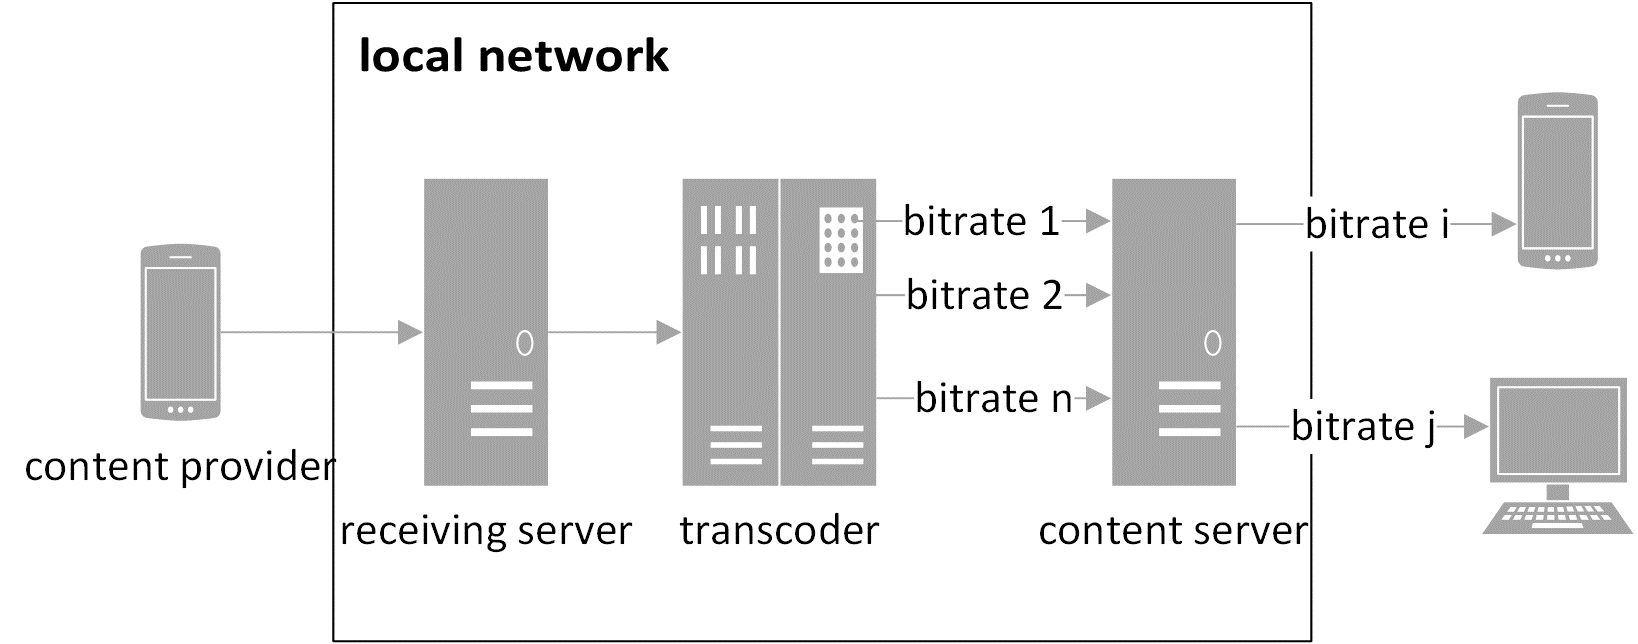
\includegraphics[width = 1.0\linewidth]{clip/07.png}
	\vspace{10pt}
	\caption{通用的手机直播系统模型\label{fig:07}}
	\vspace{10pt}
\end{figure}

容易看出,在这样的直播系统中,依次有两个传输阶段。第一个是上传阶段,即内容产生方将录制的视频传给服务器;第二个是分发阶段,即视频数据发送给观看者。第二个阶段与点播系统类似,而且服务器端转码成多码流正是为了提供这一阶段传输的码率自适应性。本文主要关注的是第一个阶段,即上传阶段的码率自适应问题。

为了提供高质量的直播视频流,内容产生方理论上应该上传尽可能高码率的视频。然而高码率可能导致数据传输时间过长,造成接收端的播放中断。因此,在带宽变化的情况下,而内容产生方一方面需要尽可能利用网络吞吐量传输高质量的视频,另一方面还要保证接收端的流畅播放。与此同时,由于UGC直播应用大多具备交互功能,所以延迟需要控制在一个可以接受的范围。这就是我们在内容产生方设计的上传码率自适应模块所要达到的目标。

为简单起见,我们假设服务器具有快速的内部操作,同时接收端通过稳定高效地网络与服务器进行连接,这意味着服务器和接收端的视频流与内容产生方和服务器的视频流保持同步。这个假设对我们的研究重点没有影响。于是我们将传输架构简化成如图\ref{fig:08}所示。内容产生方的编码器将输入视频压缩之后传递给基于TCP的应用层协议。经过各层协议的封装,数据被传递到网络进行实际传输。在接收端经过一个逆向过程之后,数据输入到解码器进行解码,然后在播放器中进行渲染。与此同时,在发送方的自适应控制模块每隔特定的周期对传输信息进行检查,并采用码率自适应算法所给出的结果对编码器参数进行调整。

现在几乎所有的UGC直播应用采用的都是RTMP协议,而RTMP协议是基于TCP的,所以在我们的研究中,主要考虑的是传输层协议为TCP的情况。接下来首先详细分析直播中的传输过程,建立一个多缓冲区模型。然后根据缓冲区模型提供的系统状态信息来设计码率自适应算法。

\begin{figure}[h]
	\centering
	\vspace{10pt}
	\vspace{10pt}
	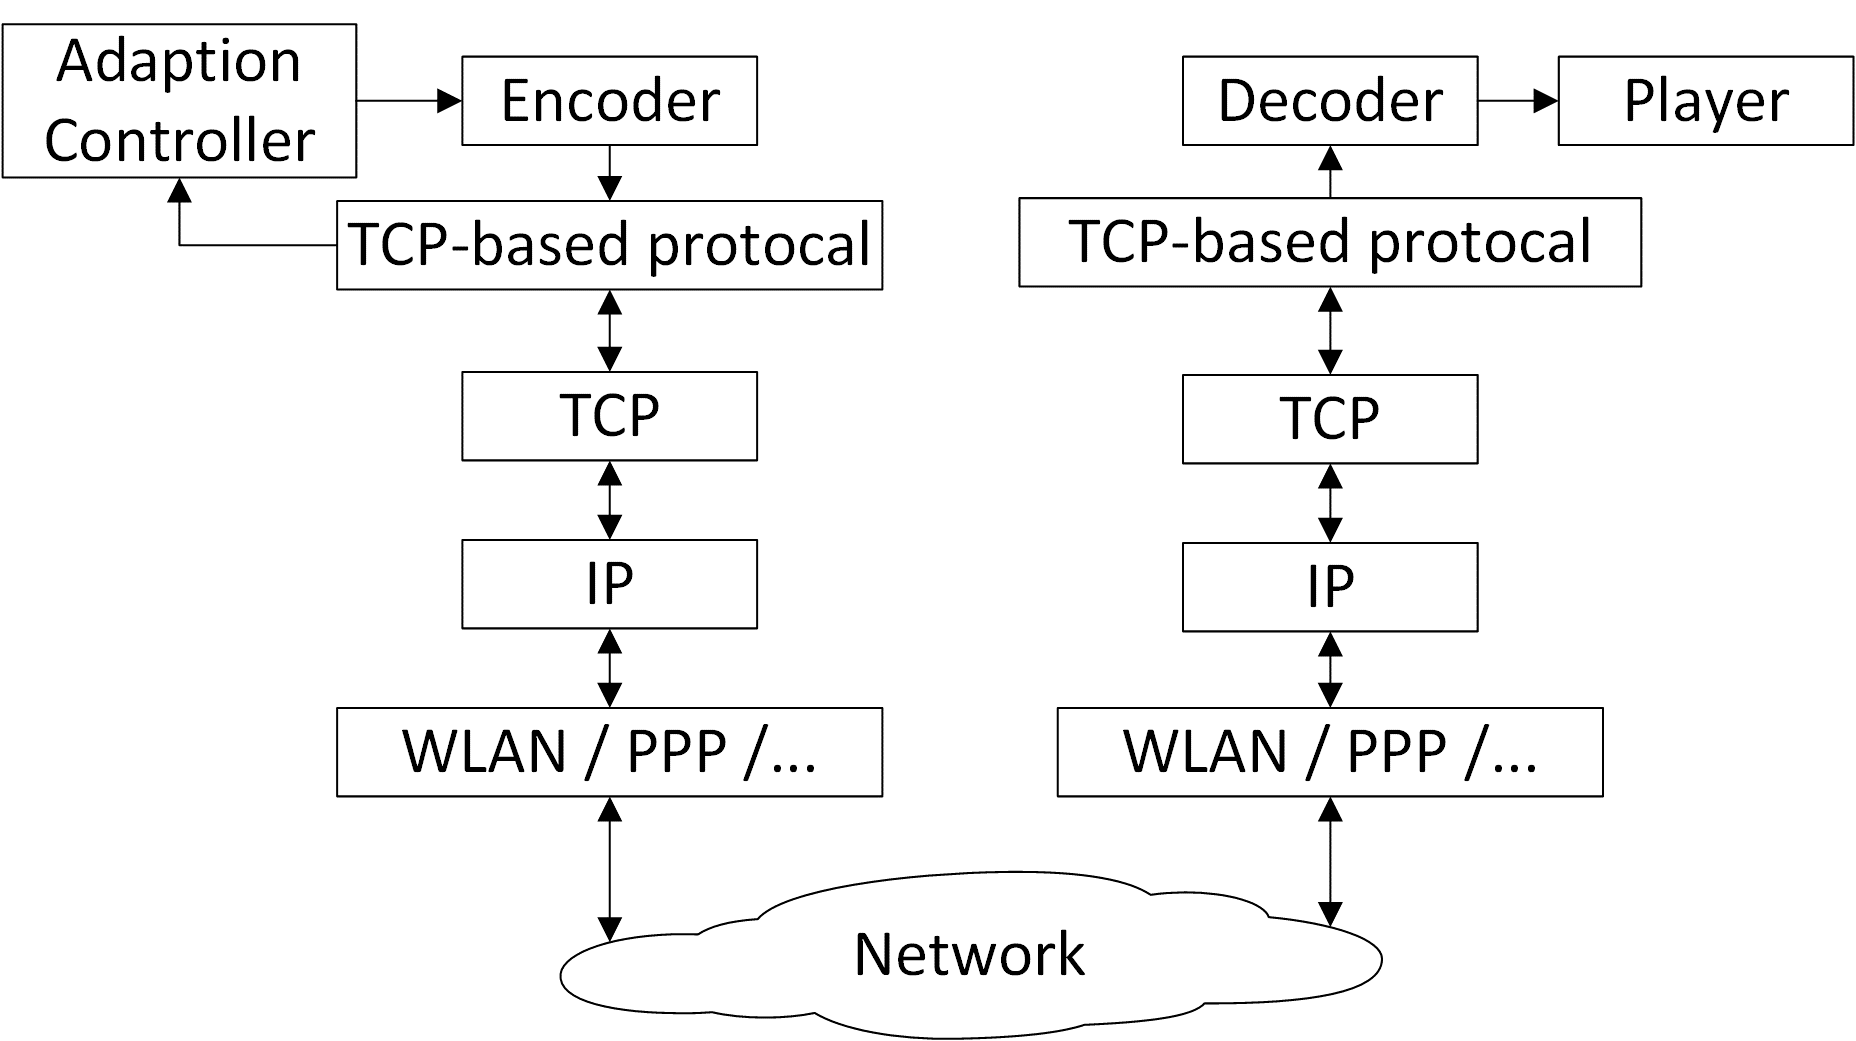
\includegraphics[width = 0.9\linewidth]{clip/08.png}
	\vspace{10pt}
	\caption{简化的直播系统传输架构\label{fig:08}}
	\vspace{10pt}
\end{figure}

\section{直播中的多缓冲区模型}

本节介绍所提出的多缓冲区模型。我们把直播中的传输过程视为几个不同的数据缓冲区的串联。这些缓冲区的状态可以被用来评估当前的网络状况,从而为码率自适应提供信息。

\subsection{TCP缓冲区}

TCP是一种网络传输层协议,属于互联网协议栈中的重要组成部分。在传输过程当中,TCP协议采用了一种滑动窗口机制来保证可靠性,同时控制流量。为了实现滑动窗口机制,存在一个TCP发送缓冲区(TCP Sending Buffer,TSB)来缓存将要发送的数据同时维护滑动窗口;对应的有一个TCP接收缓冲区(TCP Receiving Buffer,TRB)来缓存接收成功但未被上层协议获取的数据。TSB中的数据收在到接收确认之后才会被移除,而TRB中的数据在被上层协议获取之后才会被移除。这些缓冲区一般是由协议内部实现的,应用程序很少干涉。

\subsection{应用层发送缓冲区}

在TCP协议的数据接收端,只有当TRB中存在足够空间的时候,数据才能被接收,这时传输才会真正发生。反之,在数据发送端,只有当TSB中存在足够空间的时候,其上的应用层协议才能够将数据放入TSB。否则,上层协议的进程将会被阻塞,等待TSB中缓存的数据被移除。我们将应用层每次向TSB写入数据的单位定义为“数据段”(data segment),以方便后续的讨论。

我们将第$i$次阻塞时间表示为$\varDelta t(i)$,将直播系统中视频的帧率表示成$f$,并假设每一个数据段内的视频帧数为$n$。如果对于所有的$i$,都满足$\varDelta t(i) \le n/f$,那么这是较为理想的情况,因为不存在发送数据的积累。否则,在产生阻塞的时候需要采用应用层发送缓冲区(Application-layer Sending Buffer, ASB)来缓存持续产生的视频数据。当TSB中产生足够的空间的时候,ASB队列头部的数据将会被移出进行发送。我们定义ASB的长度为其中数据段的数量,在大多数情况下我们期望它是一个较小的值。在通常情况下,存在ASB的最大长度。如果ASB达到了最大长度,后面到来的数据段将会被丢失。ASB长度上限的设置是一种通用的限制延迟的方法。

\subsection{播放缓冲区}

由于网络带宽和延迟的抖动,接收方收到数据并不是完全匀速的。在这种情况下,为了保持连续的播放,几乎所有播放器都会设置一个播放缓冲区(PB),它从TRB中获取数据,并按照固定的速率将数据解码并显示。当PB的长度的为0时,视频停止播放直到PB的长度增长到一个固定值。我们称这个值为初始值,并表示为$S_0$。在很多系统中,播放缓冲区都非常有用,它弥补了短时间视频码率和网络带宽的不匹配,有效减少了视频中断的现象。通常情况下,$S_0$就是PB的最大长度。当PB长度达到$S_0$之后,再收到的数据段在接收端将被丢弃。

图\ref{fig:20}展示了接收端的数据曲线。$G(t)$表示在时间$t$之前在内容产生方生成的数据段的数量,因此$G(t) = \mu t$,其中$\mu$是一个常量,表示数据段生成的速率。$A(t)$和$P(t)$表示在接收端接收到和播放的数据段的数量,图中有$S(t) = A(t) - P(t)$。第一个数据段在经过传输延迟$d_t$之后到达接收端,PB开始接收到数据。我们假设在时间$t_0$,第一次使得$S(t_0)=S_0$,开始进行播放。$t_0$可以看做播放延迟,我们表示成$d_p$。因此,存在$S(t) \le \mu (d_p - d_t)$。当$S(t)$减小到$0$,播放终止,直到$S(t)$重新增长到$S_0$。

\begin{figure}[t]
	\centering
	\vspace{10pt}
	
\includegraphics[width = 1.0\linewidth]{clip/20.png}
	\vspace{10pt}
	\caption{直播系统接收端数据关系\label{fig:20}}
	\vspace{10pt}
\end{figure}

\subsection{多缓冲区模型分析}

如上文所讨论的,在直播传输过程中有四个缓冲区:TCP发送缓冲区(TSB)、TCP接收缓冲区(TRB)、应用层发送缓冲区(ASB)、播放缓冲区(PB),他们组成了多缓冲系统。图\ref{fig:21}显示了多缓冲区模型的结构图,其中$G(t)$、$P(t)$以及$A(t)$的定义与上一小节讨论的相同,$D(t)$表示在时间$t$之前进入TSB的数据段数量。我们使用$S_b(t)$表示在时间$t$存在于缓冲区$b$的数据段的数量,则存在:

\begin{equation}
\label{eq:mm-1}
S_{ASB}(t)=G(t)-D(t),
\end{equation}

\begin{equation}
\label{eq:mm-2}
S_{TSB}(t)=D(t)-A(t),
\end{equation}

\begin{equation}
\label{eq:mm-3}
S_{TRB}(t)=A(t)-A(t)=0,
\end{equation}

\begin{equation}
\label{eq:mm-4}
S_{PB}(t) =A(t)-P(t),
\end{equation}

\begin{equation}
\label{eq:mm-5}
S_{ASB}(t)+S_{TSB}(t)+S_{TRB}(t)+S_{PB}(t)=G(t)-P(t).
\end{equation}

公式\ref{eq:mm-3}表示TRB的大小为0,这是因为在RTMP协议实现中TRB内一旦累积到一个完整的数据段,该数据段都会迅速被应用层获取。当接收端连续正常播放视频的时候,存在
\begin{equation}
\label{eq:mm-6}
G(t)-P(t)=\phi,
\end{equation}
其中$\phi$是一个常量,反映了播放延迟。将公式(\ref{eq:mm-3})、(\ref{eq:mm-6})代入公式(\ref{eq:mm-5}),我们可以得到:
\vspace{10pt}
\begin{equation}
\vspace{10pt}
\label{eq:mm-7}
S_{ASB}(t)+S_{PB}(t)=\phi-S_{TSB}(t).
\end{equation}

当$S_{ASB}(t)=0$时,由公式(\ref{eq:mm-1})和(\ref{eq:mm-2})可知,$S_{TSB}(t)$的长度由$A(t)$决定(因为$G(t)$以匀速增长),它反映了网络状况。当$S_{ASB}(t)>0$时,意味着在发送数据到TSB时发生了阻塞,TSB一直处于充满状态,$S_{TSB}(t)$达到了上限,我们表示为$\alpha$。在这种情况下,公式(\ref{eq:mm-7})成为:
\vspace{10pt}
\begin{equation}
\vspace{10pt}
\label{eq:mm-8}
S_{ASB}(t)+S_{PB}(t)=\phi-\alpha=\delta.
\end{equation}
这意味着可以通过ASB的变化来控制和估计PB的变化。当$0 < S_{PB}(t) \le S_0$的时候,播放是连续的;这可以通过保持$\delta - S_0 \le S_{ASB}(t) < \delta$来实现,其中$\delta \ge S_0$。为了实现最小的延迟,$\delta$期望被设置为$S_0$。

\begin{figure}[t]
	\centering
	
\includegraphics[width = 1.0\linewidth]{clip/21.png}
	\caption{多缓冲区模型结构图\label{fig:21}}
\end{figure}

$S_{ASB}(t)$作为应用层的信息很容易获取,我们下面基于它在内容产生方设计一个码率自适应算法来实现高效的上传过程。


\section{码率自适应算法}

在这一节中,我们详细介绍所提出的直播系统中上传过程的码率自适应算法。具体来讲,我们希望自适应过程实现以下几个目标:(1)接收端能够连续播放;(2)传输和当前吞吐量匹配的最高视频质量;(3)尽可能低的延迟;(4)在快速波动的网络状况下灵敏地自适应;(5)方法具有通用性,能够容易地实现。

为实现目标(5),我们的方法建立在通用的基于TCP的模型上,并采用了方便获取的应用层信息。对于目标(3)和(4),我们考虑了最小可调度单元(Minimum Schedulable Data Unit,MSDU)的大小。对于目标(1)和(2),我们利用了PID控制思想的优势,通过选取系统变量和控制目标,能够动态地将系统保持在理想状态。

\subsection{最小可调度单元}

最小可调度单元(MSDU)指的是为系统能够完整传输或丢弃的最小的单位。在我们所讨论的系统中,MSDU就是上面提到的数据段。数据段的小大可以在两个方面对系统产生影响:(1)传输延迟,数据段中的数据越多,第一个数据段完整到达接收端需要的时间就越长;(2)自适应的灵敏度,一次自适应调整只有在当前正进行的数据段传输过程结束之后才会起作用。因此我们期望数据段的大小能够最小。

在基于DASH的方案中,数据段通常是一个图像组(GOP)\supercite{Cicco2011}。一个GOP可以单独播放,当一个GOP被丢弃时,对其他的GOP没有影响。通常一个GOP的持续时间是1到5秒。而在我们的方法中,我们将数据段(也就是MSDU)设置为视频帧,这样可以将传输延迟最小化,以及将自适应的灵敏度最大化。如果在缓冲区极端情况下当一帧被丢弃时,我们需要丢弃其同一个GOP中后续的帧,这样才不会带来解码的错误。

\subsection{过程变量选取}

利用PID方法进行码率自适应的关键在于选取一个能够反映传输状况的过程变量。根据上面对多缓冲区模型的分析,基于TCP的直播系统在传输过程中对内容产生方最重要的信息是ASB内的数据长度,即$S_{ASB}(t)$(在时刻$t$的值),它能够直接反映视频码率和吞吐量之间的匹配情况。当视频码率高于当前的吞吐量时,该缓冲区内的数据长度趋向于增大,否则保持相对稳定或者减小为0。

根据自适应的目标,首先需要确保流畅的播放,如上面所讨论过的,这可以通过保持$\delta - S_0 \le S_{ASB}(t) < \delta$来实现。为了实现最低延迟,我们将$\delta$设定为$S_0$。因此,ASB的大小应当被控制在$S_0$以内,否则将会出现播放中断。

与此同时,我们系统网络带宽被充分利用,这可以通过使TSB充满来实现。如上面所讨论过的,当$S_{ASB}(t)>0$时,TSB为充满状态,$S_{TSB}(t)$达到了上限。

综合以上两点,$S_{ASB}(t)$的理想状态应为:
\vspace{10pt}
\begin{equation}
\vspace{10pt}
\varepsilon \le S_{ASB}(t) \le \varepsilon+\theta,
\end{equation}
其中$\varepsilon$以及$\theta$是很小的常量,并且$\varepsilon+\theta<S_0$。

根据上述分析,我们定义系统的过程变量为$S_{ASB}(t)$,它代表在时间$t$时ASB的大小,其目标值为$\varepsilon$。程序将周期性地自动检查ASB,获取当前的过程变量值,并采用基于PID的自适应算法来调整视频码率。

然而,如果网络吞吐量在一个小的范围频繁波动,将使得该过程变量值不稳定而且相对随机,导致不必要的频繁调整。为了消除这样的随机性,我们将过程变量的定义修改为$\overline{S_{ASB}(t)}$,它表示在时刻$t$之前的一个检查间隔时间段$\tau$内$S_{ASB}(t)$的平均值。它可以表示为:
\vspace{10pt}
\begin{equation}
\vspace{10pt}
\label{eq:asb}
\overline{S_{ASB}(t)} = \dfrac{1}{\tau} \int_0^\tau {S_{ASB}(t)}\: .
\end{equation}

另一方面,为了减小不稳定性,我们对通用PID模型中的误差也进行量化,将其表示为:
\vspace{10pt}
\begin{equation}
\vspace{10pt}
e(t) = step \times \left \lfloor\dfrac{\varepsilon - \overline{S_{ASB}(t)}}{step} \right \rfloor,
\end{equation}
其中$step$是量化步长,并且$step<\varepsilon$。

\subsection{算法详情}

为了计算$\overline{S_{ASB}(t)}$,我们会维护一个发送状态列表。每一个数据段(视频帧)从ASB发送出去的时候,我们都会记录下此时的ASB长度,放入列表中。当每一个检查间隔时间点到来时,通过这个列表来计算ASB长度的平均值。

对于直播应用来讲,由于发送的码流是实时生成的,所以调整码率时直接改变编码器参数以改变生成的码率即可,不需要涉及码流截取等数据源端的操作。但是,质量等级的概念仍然需要,它在这里变成了改变码率的单位。控制模型直接采用原始PID中的做法,用过程变量$\overline{S_{ASB}(t)}$和控制目标$\varepsilon$的差值来计算比例、积分、微分这几个部分。这个差值从物理意义上来看单位是数据段,当用它计算得到控制器输出时,该输出需要根据实际意义转换成码率的调整量。

具体的算法流程如Algorithm\ref{algo:control-live}所示。PID中三个增益参数的选取和调优可以参见上一章中的相关内容,这里不再详述。

\vspace{10pt}
\begin{algorithm}
	\vspace{10pt}
	\caption{基于PID的直播码率自适应算法}
	\label{algo:control-live}
	\begin{algorithmic}
		\WHILE{is\_started}
		\STATE wait for check period
		\STATE average\_s = get\_average\_ASB\_size()
		\STATE error = get\_error(average\_s, set\_point)
		\IF{error == 0}
			\STATE last\_error = error
			\STATE summation = 0
		\ELSE
			\STATE summation = summation + error
			\STATE difference = error – last\_error
			\STATE output = $K_p$*error + $K_i$*summation + $K_d$*difference
			\STATE change\_bitrate(output)
		\ENDIF
		\ENDWHILE
	\end{algorithmic}
	\vspace{10pt}
\end{algorithm}
\vspace{10pt}
	
\section{实验结果}

\subsection{实验配置}

为了对基于PID的直播系统内容发送码率自适应方法进行测试,我们实现了一个实际的手机视频直播系统。根据图\ref{fig:07},这个系统包含三个部分:内容产生方、中转服务器、播放终端。

我们选择业界已经广泛使用的RTMP协议作为应用层流媒体协议,具体实现采用了第三方开源的代码库librtmp\footnote{http://rtmpdump.mplayerhq.hu/librtmp.3.html}。我们在Android平台上实现了内容产生和上传的程序,其中采用了开源软件x264\footnote{http://www.videolan.org/developers/x264.html}作为视频编码器,并集成了本文提出的码率自适应算法。我们用nginx-rtmp-module\footnote{https://github.com/arut/nginx-rtmp-module}帮助完成了中转服务器的搭建。播放终端采用了开源播放器ffplay\footnote{https://ffmpeg.org/},它可以播放RTMP协议的流媒体并对播放缓冲区长度进行设置。

\begin{figure}[!t]
	\centering
	\vspace{10pt}
	\subfloat[1Mbps的固定带宽的实验结果]{\label{fig:09-1}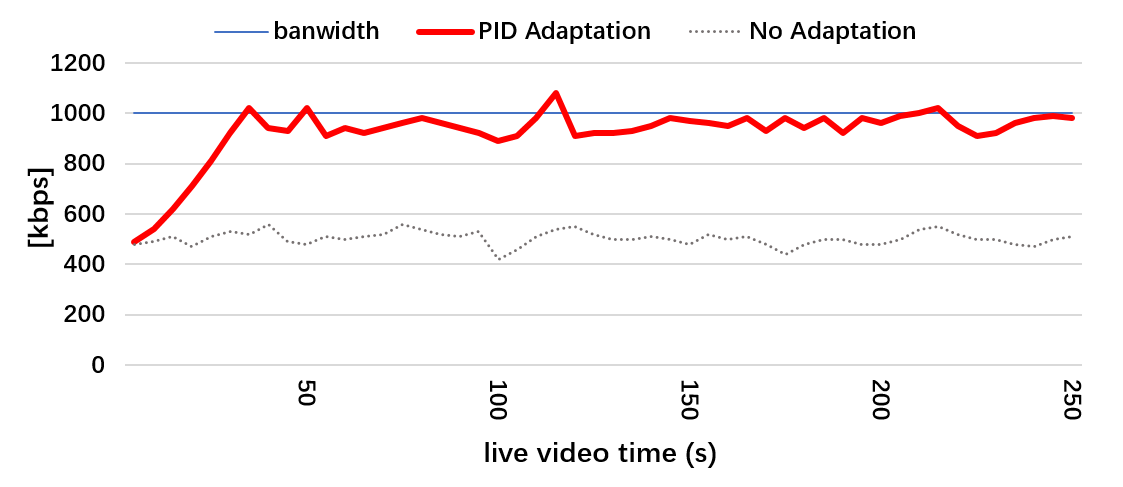
\includegraphics[width=0.9\textwidth]{clip/09-1m.png}} \\
	\subfloat[长周期波动带宽的实验结果]{\label{fig:09-2}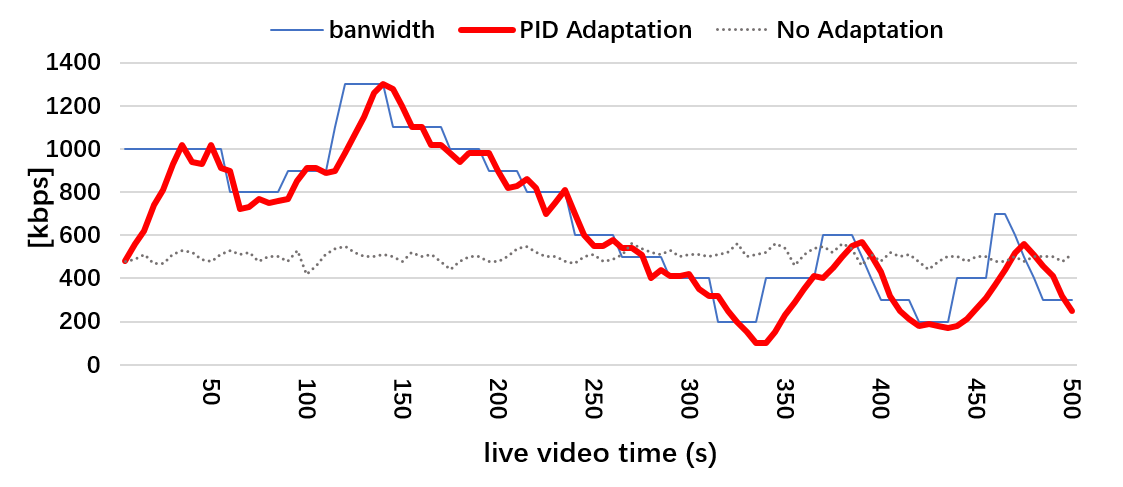
\includegraphics[width=0.9\textwidth]{clip/09-2m.png}} \\
	\subfloat[短周期波动带宽的实验结果]{\label{fig:09-3}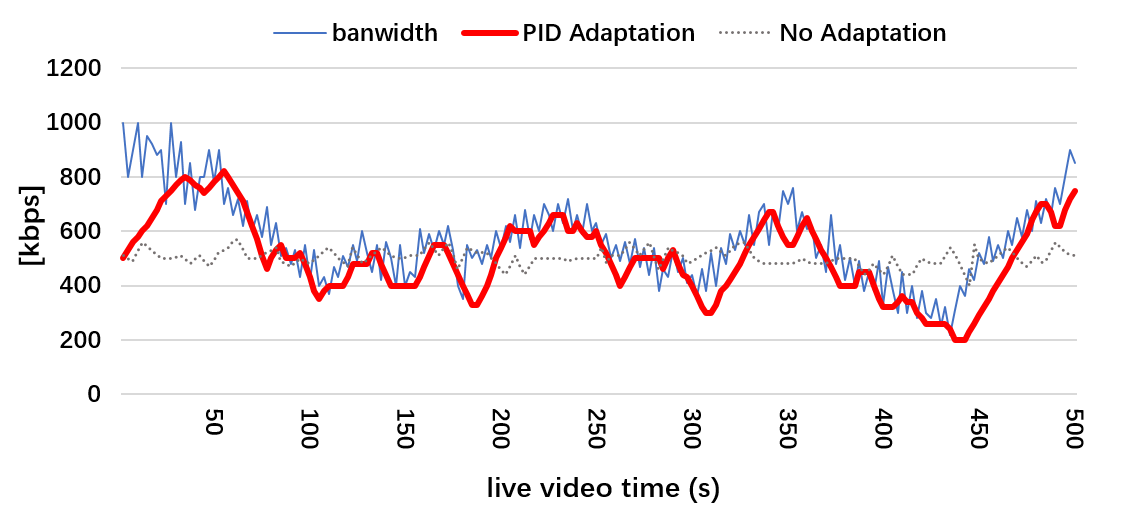
\includegraphics[width=0.9\textwidth]{clip/09-3m.png}}
	\caption{直播系统在不同测试条件下码率随时间变化的情况}
	\label{fig:09}
\end{figure}

\begin{figure}[!t]
	\centering
	\vspace{10pt}
	\subfloat[1Mbps的固定带宽的实验结果]{\label{fig:14-1}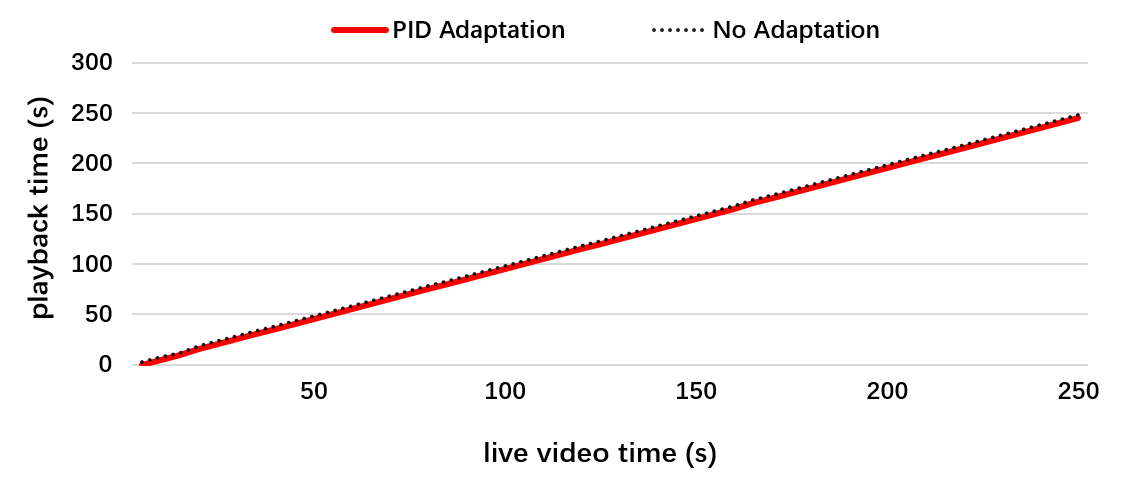
\includegraphics[width=0.9\textwidth]{clip/14-1m.png}} \\
	\subfloat[长周期波动带宽的实验结果]{\label{fig:14-2}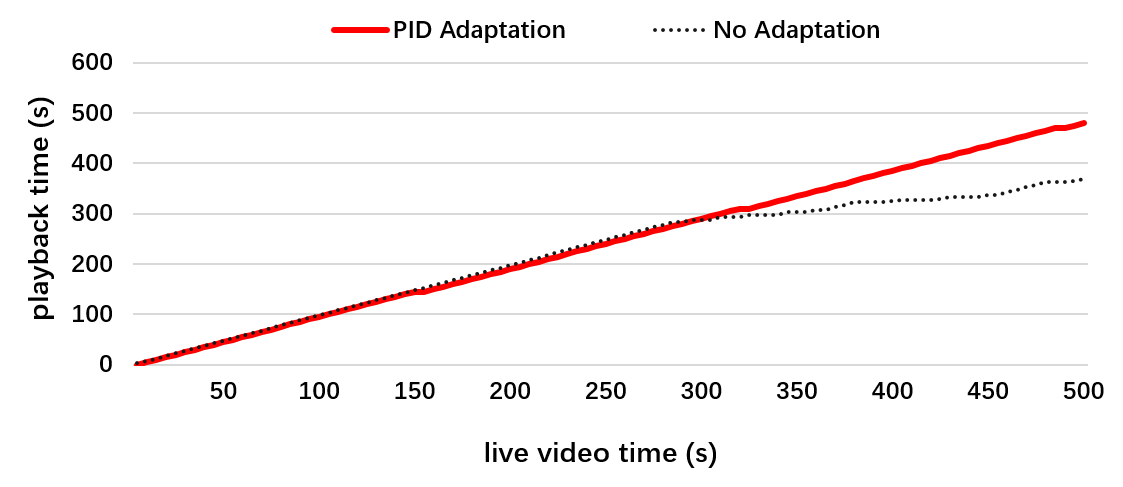
\includegraphics[width=0.9\textwidth]{clip/14-2m.png}} \\
	\subfloat[短周期波动带宽的实验结果]{\label{fig:14-3}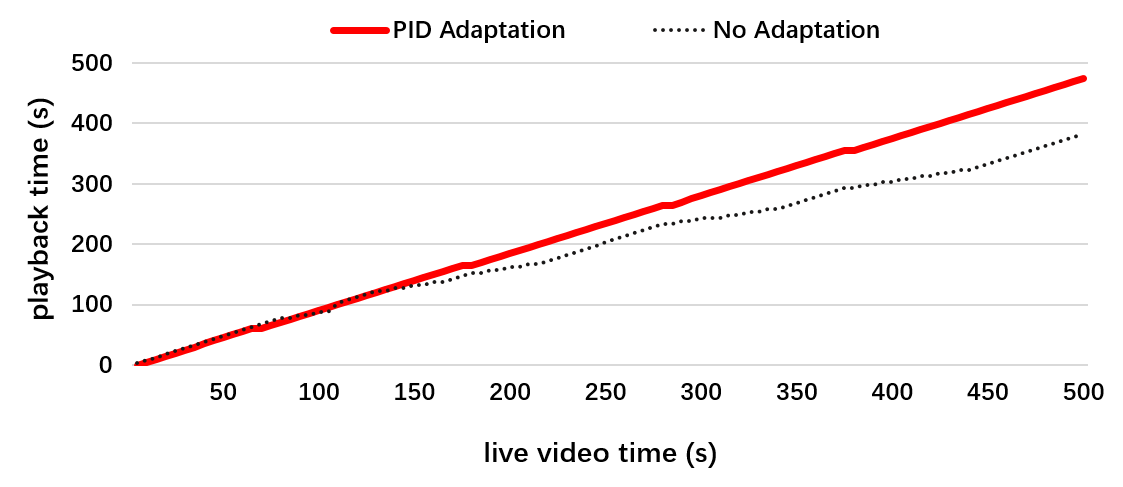
\includegraphics[width=0.9\textwidth]{clip/14-3m.png}}
	\caption{直播系统在不同测试条件下播放时间占比的变化情况}
	\label{fig:14}
\end{figure}

在我们的实验中,我们通过动态改变内容产生方所连接的路由器所允许的最大带宽来模拟出波动的网络状况。视频的采集帧率设置为15 FPS;ASB的最大长度为150,PB最大长度$S_0$为60,过程变量$\overline{S_{ASB}(t)}$的控制目标值$\varepsilon$为15,误差量化步长$step$为5(这些值的单位是数据段的个数,每个数据段为一个视频帧);改变码率的单位为20kbps,初始码率为500kbps;对过程变量的检查间隔为2秒。我们调节得到的PID控制参数$K_p$、$K_i$和$K_d$分别为0.8,0.13以及0.07。

我们在3种条件下进行了测试:(1)固定带宽(Constant Bandwidth,CB),带宽固定为1Mbps;
(2)长周期波动带宽(Long-Term Bandwidth Variation,LTBV),带宽每隔40秒变化一次,在200kbps到1.4Mbps之间波动;(3)短周期波动带宽(Short-Term Bandwidth Variation,STBV),在200kbps到1.4Mbps之间随机波动。

\subsection{结果分析}

测试结果参见图\ref{fig:09}、\ref{fig:14}和表\ref{tab:live-bandwidth}、\ref{tab:live-playtime}。由于移动设备上的UGC视频直播应用刚兴起不久,我们暂未发现有针对这一传输模式的研究工作可供对比。因此,在实验中我们只与不进行码率调整的系统进行了比较。

从图\ref{fig:09-1}中可以看出,我们提出的自适应方法使得码率在35秒以内保持上升,直到趋近带宽。从图\ref{fig:09-2}和\ref{fig:09-3}可以看出,通过PID自适应算法的调整,在一个合理的延迟之内,码率和波动的带宽基本保持同步,而且系统对带宽的频繁变化进行了一定的平滑。如表\ref{tab:live-bandwidth}所示,码率不进行调整时带宽占用率较低,而我们提出的算法对于条件(1)、(2)和(3)分别将带宽占用率提高到92.1\%、88.9\%以及87.1\%。

从图\ref{fig:14-1}可以看出,在带宽固定的情况下,对于进行自适应码率调整和未进行码率调整的视频流,播放基本都是连续的。但从图\ref{fig:14-2}和\ref{fig:14-3}可以看出,未进行码率调整的视频流的播放过程被频繁地中断,而进行码率调整的视频流的播放过程在大部分时间是连续的。如表\ref{tab:live-playtime}所示,我们所提出的方法对于条件(2)和(3)分别将播放时间占比提高到97.3\%和96.1\%,因此显著提高了播放连续性。

总之,加入PID码率自适应算法比不进行码率调整的直播效果有所改善。

\begin{table*}
	\centering
	\vspace{10pt}
	\caption{直播系统实验中的带宽利用率}
	\label{tab:live-bandwidth}
	\begin{tabular}{c|*{2}{p{1.0cm}<{\centering}|}{p{1.0cm}<{\centering}}}
		\hline\hline
		& CB & LTBV & STBV \\ \hline
		自适应调整码率  & 92.1\% & 88.9\% & 87.1\% \\ \hline
		不进行调整 & 50.4\% & 64.7\% & 80.3\% \\ \hline
	\end{tabular}
\end{table*}

\begin{table*}
	\centering
	\vspace{10pt}
	\caption{直播系统实验中的播放时间占比}
	\label{tab:live-playtime}
	\begin{tabular}{c|*{2}{p{1.0cm}<{\centering}|}{p{1.0cm}<{\centering}}}
		\hline\hline
		& CB & LTBV & STBV \\ \hline
		自适应调整码率  & 100\% & 97.3\% & 96.1\% \\ \hline
		不进行调整 & 100\% & 73.4\% & 71.5\% \\ \hline
	\end{tabular}
\end{table*}

\section{本章小结}

本章提出了一种针对视频直播系统中数据上传阶段的码率自适应算法。首先采用多缓冲模型来详细分析了整个传输过程,并根据缓冲区的状态来评估网络状况。在此基础上设计了一种基于PID的码率调整策略,能够灵敏地调节视频码率来匹配当前的网络带宽,从而在保证流畅播放的情况下提供最高能达到的视频质量。在我们实现的手机视频直播系统中的测试结果表明,所提出的算法提高了带宽的利用率,并改善了带宽波动情况下播放的流畅性。